% easychair.tex,v 3.3 2013/09/17
%
% Select appropriate paper format in your document class as
% instructed by your conference organizers. Only withtimes
% and notimes can be used in proceedings created by EasyChair
%
% The available formats are 'letterpaper' and 'a4paper' with
% the former being the default if omitted as in the example
% below.
%
\documentclass{easychair}
%\documentclass[debug]{easychair}
%\documentclass[verbose]{easychair}
%\documentclass[notimes]{easychair}
%\documentclass[withtimes]{easychair}
%\documentclass[a4paper]{easychair}
%\documentclass[letterpaper]{easychair}

% This provides the \BibTeX macro
\usepackage{doc}
\usepackage{makeidx}

% In order to save space or manage large tables or figures in a
% landcape-like text, you can use the rotating and pdflscape
% packages. Uncomment the desired from the below.
%
% \usepackage{rotating}
% \usepackage{pdflscape}

% If you plan on including some algorithm specification, we recommend
% the below package. Read more details on the custom options of the
% package documentation.
%
% \usepackage{algorithm2e}

% Some of our commands for this guide.
%
\newcommand{\easychair}{\textsf{easychair}}
\newcommand{\miktex}{MiK{\TeX}}
\newcommand{\texniccenter}{{\TeX}nicCenter}
\newcommand{\makefile}{\texttt{Makefile}}
\newcommand{\latexeditor}{LEd}

%\makeindex

%% Document
%%
\begin{document}

%% Front Matter
%%
% Regular title as in the article class.
%
\title{Big Astrophysical Data Visualisation on the MIC architecture}

% \titlerunning{} has to be set to either the main title or its shorter
% version for the running heads. When processed by
% EasyChair, this command is mandatory: a document without \titlerunning
% will be rejected by EasyChair

\titlerunning{The {\easychair} Class File}

% Authors are joined by \and. Their affiliations are given by \inst, which indexes
% into the list defined using \institute
%
\author{
  Claudio Gheller\inst{1}  %\thanks{Designed and implemented the class style}
\and
  Timothy Dykes\inst{2}   %\thanks{Masterminded EasyChair and created versions}\\
\and
  Mel Krokos\inst{2}  %\thanks{Did numerous tests and provided a lot of suggestions}
\and
  Marzia Rivi\inst{3} %\thanks{Changed author list format.}\\
}

% Institutes for affiliations are also joined by \and,
\institute{
  CSCS-ETHZ,
  Lugano, Switzerland\\
  \email{cgheller@cscs.ch}
\and
   University of Portsmouth,
   Portsmouth, U.K.\\
   \email{timothy.dykes@myport.ac.uk, mel.krokos@port.ac.uk}\\
\and
   University of Oxford,
   Oxford, U.K.\\
   \email{rivi@physics.ox.ac.uk}\\
 }
%  \authorrunning{} has to be set for the shorter version of the authors' names;
% otherwise a warning will be rendered in the running heads. When processed by
% EasyChair, this command is mandatory: a document without \authorrunning
% will be rejected by EasyChair

\authorrunning{Mokhov, Sutcliffe, Voronkov and Gough}


\clearpage

%%%%%%%%%%%%%%%%%%%%%%%%%%%%%%%%%%%%%%%%%%%%%%%%%%%
\maketitle
%%%%%%%%%%%%%%%%%%%%%%%%%%%%%%%%%%%%%%%%%%%%%%%%%%%

\begin{abstract}
.....................
\end{abstract}

\pagestyle{empty}


%------------------------------------------------------------------------------
\section{Introduction}
\label{sect:introduction}

The scientific data volume produced by experiments, observations and numerical simulations 
is increasing exponentially with time. This is true for any scientific domain, but in 
particular for astrophysics. Next generations of telescopes and antennas are expected to produce
enormous amount of data. The Square Kilometer Array project (REF), for instance, will 
generate an exabyte of data every day, twice the information currently exchanged on 
the internet on a daily basis and 100 times more information then the CERN LHC (REF) experiment
produces. At the same time, computer simulations represent an invaluable instrument for 
astrophysicists to validate theories and compare to observations through numerical experiments.
The ultimate cosmological simulations (REF), performed using sophisticated N-body codes (REF), 
could describe the details of the evolution of the universe up to the present time, following the behaviour of 
gravitating matter represented by a hundred billion particles. These runs produce output files 
whose size is of the order of tens of terabytes each. The fast technological progresss 
of supercomputing systems will soon lead to simulations producing outputs with size of the order of 
the petabyte or more. 

Size does not represent the only challenge posed by scientific data. Is also essential to 
effectively extract all the information hidden in the sea of bytes represented by each 
single data file. Software for data mining and analysis is often highly computationally
demanding and ultimately unusable on large datasets.  

Visual exploration and discovery represents an outstanding aid to big data processing, 
e.g. by providing scientists with
prompt and intuitive insights enabling them to identify interesting 
characteristics and thus define regions of interest within which to apply time-consuming 
methods. Additionally, they can be a very effective way in discovering and
understanding correlations, associations and data patterns, or in identifying unexpected behaviours
or even errors. Visualization is also an effective means for communicating scientific results not
only to researchers but also to members of the general public.
However, also visualization tools require high performance computing (hereafter HPC) resources, to 
fulfil the requirements posed both from data size and from the need of having
fast (if not real-time) rendering.

This paper will show how the Splotch software (REF), our ray-casting algorithm for
effectively visualizing large-scale, particle-based datasets, addresses these issues, 
providing high quality graphic outputs, processing data of, ideally, any size, 
efficiently exploiting a broad variety of HPC systems. 
In particular, we will describe the work accomplished to enable Splotch to 
run on the Intel PHI (REF) architecture, taking advantage of the Many Integrated Core (hereafter MIC) accelerator,
which is expected to provide, on suitable classes of algorithms, outstanding performance 
with power consumption being comparable to standard CPUs. 
We will present the MIC implementation and optimisations, performance tuning,
benchmarks carried out, and the resulting performance measurements, comparing that of an OpenMP
based implementation running on multiple cores of a single CPU. A brief overview of this implementation
will also be given, referring to [REF] for further details.

\section{Splotch Overview}
\label{sect:overview}

\noindent
Contents:

\noindent
- Standard brief overview of Splotch workflow 


\subsection{MPI and
 OpenMP Implementations}
\label{sect:mpiopenmp}

\noindent
Contents:

\noindent
- Describing how OpenMP implementation works for reference when building upon this for the MIC implementation.

\noindent
- Describing how MPI implementation works for reference when discussing how MPI is used to increase MIC performance.

\noindent
- Mention GPU implementation with reference, no need for details

\section{Splotch on the MIC}
\label{sect:micsplotch}

The MIC based implementation of Splotch exploits both OpenMP and MPI in order to fully exploit the many core 
programming paradigm necessary to take advantage this architecture. This section gives a brief overview of the 
Xeon Phi, and the steps taken to modify and optimise Splotch to make effective use of this hardware.

\subsection{Overview of the MIC Architecture}
\label{sect:mic}

The core ideal behind the MIC micro-architecture is obtaining a massive level of parallelism for high throughput 
performance in power restricted cluster environments. To this end Intel's flagship MIC product, the Xeon Phi, 
contains roughly 60 cores on a single chip – dependant on the model. Each core has access to a 512 KB private 
fully coherent L2 cache, memory controllers and the PCIe client logic provide access to up to 8 GB of GDDR5 
memory, and a bi-directional ring interconnect brings these components together. The cores are in-order, however 
up to 4 hardware threads are supported to mitigate the latencies inherent with in-order execution. The Vector 
Processor Unit (hereafter VPU) is worthy of note due to the utilisation of an innovative 512 bit wide SIMD 
capability, allowing 16 single precision (SP) or 8 double precision (DP) floating point operations per cycle, 
support for fused-multiply-add operations increased this to 32 SP or 16 DP floating point operations per cycle. 

The Xeon Phi acts as a coprocessor for a standard Intel Xeon processor connected via PCIe, and there are various 
modes of execution on a system utilising one or more Xeon Phi coprocessors. It runs the Linux operating system, 
and so can be seen as a networked node through a virtualised TCP/IP stack over the PCIe bus. This allows a user 
to log into the node, transfer a program over and run natively, or to use the coprocessor as an MPI process alongside 
the Xeon. The ability to partition subgroups of processors allows the Phi to run multiple MPI processes at the same 
time, a technique exploited in [insert subsection number]. In addition, a heterogenous approach is possible, using 
the coprocessor to accelerate a standard CPU based algorithm by offloading sections of computation to the device using 
a small series of extensions available to both C++ and Fortran. 

An advantageous factor of programming for the Xeon Phi, as opposed to other accelerators commonly used in HPC 
environments such as GPUs, is the similarity of techniques used to exploit parallelism on both the Xeon Phi and 
regular Xeon processors. Algorithms that already utilise parallel paradigms involving OpenMP, MPI, Intel TBB, or 
Intel Cilk Plus can often be run on the Xeon Phi with little modification. While further tuning is necessary to 
fully take advantage of the new hardware, it is not a necessity to reimplement the entire algorithm.   


\subsection{MIC Implementation}
\label{sect:micimplementation}

The implementation targeting the MIC is based on the original C++ and OpenMP version of Splotch (see section 2.1). 
While the core algorithm executes on the Xeon (referred to as the host), data is transferred to the Xeon Phi (referred 
to as the device) and the majority of the computation is offloaded using the C++ pragma extensions provided by Intel 
in a syntactic style similar to OpenMP, attention has been paid to optimising parts of the algorithm to better take 
advantage of the wide SIMD capability of the Phi.


\subsubsection{Algorithm}
\label{sect:micalgorithm}

The rendering algorithm can be broken down into a series of phases illustrated by the execution model shown in [figure x]. 
A double buffered scheme has been implemented using the ability to asynchronously transfer data via a series of signal 
and wait clauses provided by the Intel extensions. This allows to minimise overhead due to transferring data to the device 
for processing, and to facilitate the rendering of datasets potentially much larger than the memory capacity available, 
discussed further in section [section number].

\medskip
\centerline{[figure illustrating execution model]}
\medskip
A necessary overhead is incurred from the outset performing various initialisations discussed further in section 4.1. In 
addition to this, the first chunk of data must be transferred to the device before the double buffering system can begin 
to compensate for data transfer times. This initial transfer is carried out asynchronously while precomputing render 
parameters such as those used in the 3d transformation, which will be static throughout the rendering process. The render 
parameters are copied to the device, which subsequently begins rendering while the next chunk of data is transferred.

The first stage of rendering is a highly parallel 3D transform and colorize performed on a per-particle basis using 
four OpenMP threads per available core, equating to roughly 240 threads assuming the current process has access to the 
whole device. [expand on this]

The second stage is not so simply parallelised, leading to more complex solution. A problem inherent in parallel 
rendering is the appearance of race conditions arising from multiple threads attempting to render to the same pixel. 
In a scene with potentially billions of particles, it is inevitable that multiple particles, potentially a vast number, 
will overlap and need to be rendered to the same pixel. [discuss this somewhere else?]

The number of available OpenMP threads are split into groups, allocating an image buffer per group large enough to hold 
the entire resulting image. Each group is assigned a subsection of the particles where 
n\_particles\_per\_group = total\_particles / n\_groups. [Latex up this equation including remainder compensation]. At this 
point each thread group acts independently, drawing the allocated subsection of particles to the allocated image, finally 
reducing all images into a single buffer when all particles of the current data chunk have been processed, a system 
conceptually similar to the MPI Splotch implementation discussed in section 2.1. The number of groups to create and 
number of threads per group can be passed in as a runtime parameter, and the chosen values should reflect consideration 
of the available number of threads and thread:core ratio. This is discussed further in section 4.1.

Subsequent to group allocation, each thread group begins independently rendering an allocated subset of particles. This 
occurs in two phases, a pre render phase and a render phase. In order to allow each thread sole access to a particular 
set of pixels, and avoid race conditions discussed previously, the image is split into 2 dimensional grid of tiles – 
the number of which is determined by a run time parameter tile\_size. The pre-render phase generates a list of particle 
indices per tile, indicating all the particles whose area of influence overlaps with the tile. In this phase each thread 
is allocated a subset of the group's allocated particles, and generates a list for each tile resulting in 
(n\_thread * n\_tile) lists. A single thread accumulates the per-thread lists to attain a single list per tile. 
Once all lists have been accumulated, phase two begins. In this phase each thread is allocated a tile, or subset of 
pixels, and renders all particles in the list associated with that tile. In this way pixels are not shared between 
threads and concurrent accesses are avoided.

Following the accumulation of each group-specific image into a single buffer, which is retained throughout the entire 
rendering process, the next chunk of data is processed until all particles have been rendered. This constant buffer is 
then copied back to the host to be written to file. 
%\medskip
%\noindent
%- Broken into sections: Initialisation/preprep, rototranslate/color, prerender, actual render, image accumulation 



\subsubsection{Optimisation}
\label{sect:micoptimisation}

\noindent
Contents:

\noindent
- Description of various optimisation methods

\noindent
- Cost of memory allocations, avoiding this

\noindent
- AoS vs SoA

\noindent
- Double buffered computation

\noindent
- Vectorization: automatic and manual

\noindent
- Use of MPI to partition Phi's cores into sections



\section{Performance Analysis}
\label{sect:performance}

\noindent
- Contents:

\noindent
- Performance analysis methods, test hardware etc


\subsection{Tuning}
\label{sect:tuning}

\noindent
- Necessary overhead (mic initilisation, omp thread initialisation - check thread stack size allocations effect on this?)

\noindent
- Thread grouping, tile size, number of mpi processes used, results

\subsection{Scalability}
\label{sect:scalability}

\noindent
- Performance tests on various sizes of data compared to CPU

\section{Discussion and Conclusions}
\label{sect:conclusions}

...

\subsection{Acknowledgments}
\label{sect:acks}

...

%------------------------------------------------------------------------------
\end{document}

% EOF


The {\easychair} class was designed according to some requirements, which
are described in Appendix~\ref{sect:easychair-requirements}.
An article that occupies approximately 15 LNCS-formatted pages
takes up approximately 14 {\easychair} pages.

\begin{figure}[tb]
        \begin{centering}
        
\includegraphics[width=0.5\textwidth]{logoEC}
        \caption{EasyChair logo}
        \label{fig:easychair-logo}
        \end{centering}
\end{figure}

%------------------------------------------------------------------------------

\subsection{Generalities}
\label{sect:generalities}

The following are the general default parameters {\easychair}
introduces into the typesetting aspect of articles. If you use
\easychair\ for proceedings or other kinds of publishing through
EasyChair, do not alter these -- papers deviating from the formatting
standards will be rejected by EasyChair.

\begin{enumerate}
\item
The default paper size is US letter. It can be explicitly set to A4
(\texttt{a4paper}) or letter (\texttt{letterpaper}) paper in the
document class entry, e.g.:\\\verb+\documentclass[a4paper]{easychair}+

\item
The print area for both letter and A4 paper sizes is 145x224 mm. This size
has been selected to allow for inexpensive printing using our current
print-on-demand publisher.

\end{enumerate}

%------------------------------------------------------------------------------
\subsection{Mathematics}
\label{sect:mathematics}

Mathematics can be done inline for simple things, e.g., an equation
$x = 0$, possibly with super and subscripts, e.g., $x^2_k \approx 27$,
Greek letters, e.g., $\alpha \cup \Theta \ne \gamma$, etc.
Larger formulae must be done using {\tt \verb|\|[}~~{\tt \verb|\|]}
bracketing, e.g.,
\[
\int_{0}^{1} x dx = \left[ \frac{1}{2}x^2 \right]_{0}^{1} = \frac{1}{2}
\]
or using {\tt \verb|\|begin\{equation\}} and {\tt \verb|\|end\{equation\}} for
numbered equations, e.g.,
\begin{equation}
e^x = \sum_{n=0}^\infty \frac{x^n}{n!} = \lim_{n\rightarrow\infty} (1+x/n)^n
\end{equation}

Use {\tt \verb|\|begin\{align*\}} and {\tt \verb|\|end\{align*\}} (or without
the {\tt *} include number) to align equations, e.g.,
\begin{align*}
x^2 + y^2 &= 1 \\
y &= \sqrt{1 - x^2}
\end{align*}

Fonts, using \verb|\matcal| and others can also be used in the math mode: $\mathcal{ALC}$.


Table~\ref{tab:ltbexample} shows an example of a table of data that was
conveniently available (i.e., the data has nothing to do with
{\easychair}) apart from being related to the research of two of its
authors.

Table~\ref{tab:ltbexample} shows an example of a table of data that was
conveniently available (i.e., the data has nothing to do with
{\easychair}) apart from being related to the research of two of its
authors.

\begin{table}[htp]
        \begin{centering}
                \begin{tabular}{lrrrrrrrr}
                \hline
                ATP System            & LTB & Avg  &Prfs & SOTA & \multicolumn{1}{c}{$\mu$} & CYC & MZR & SMO \\
                                      & /100& time & out & Con. & Eff. & /35 & /40 & /25 \\
                \hline
                Vampire-LTB 11.0      &  69 & 24.5 &  69 & 0.37 & 28.1 &  23 &  22 &  24 \\
                iProver-SInE 0.7      &  67 & 76.5 &   0 & 0.36 &  8.8 &  28 &  14 &  25 \\
                SInE 0.4              &  64 & 75.3 &  64 & 0.32 &  8.5 &  26 &  13 &  25 \\
                leanCoP-SInE 2.1      &  35 &110.8 &  35 & 0.23 &  3.2 &  23 &   1 &  11 \\
                E-LTB 1.1pre          &  18 & 63.4 &   0 & 0.21 &  2.8 &   7 &   9 &   2 \\
                EP-LTB 1.1pre         &  18 & 77.8 &  18 & 0.21 &  2.3 &   7 &   9 &   2 \\
                E-KRH'-LTB 1.1.3      &   0 &   -- &  -- &   -- &   -- &   0 &   0 &   0 \\
                \hline
                \end{tabular}
                \caption{LTB division results}
                \label{tab:ltbexample}
        \end{centering}
\end{table}


References must be provided in a {\tt .bib} file, so that \BibTeX\ can
be used to generate the references in a consistent style in a volume.
The preferred styles are {\tt plain} and {\tt alpha}.
For example, the references for this paper are generated from the
lines
\begin{verbatim}
    \bibliographystyle{plain}
    \bibliography{easychair}
\end{verbatim}
and a way to compose the entires, e.g. citing this class style~\cite{easychair-latex-class}
is below:
\tiny
\begin{verbatim}
 @misc
 {
   easychair-latex-class,
   author       = {Serguei A. Mokhov and Geoff Sutcliffe and Andrei Voronkov},
   title        = {The {\sf easychair} Class File Documentation and Guide
                   for Authors},
   year         = {2008--2011},
   howpublished = {[online]},
   note         = {Available at \url{http://easychair.org/publications/easychair.zip}}
 }
\end{verbatim}
\normalsize


\begin{verbatim}
  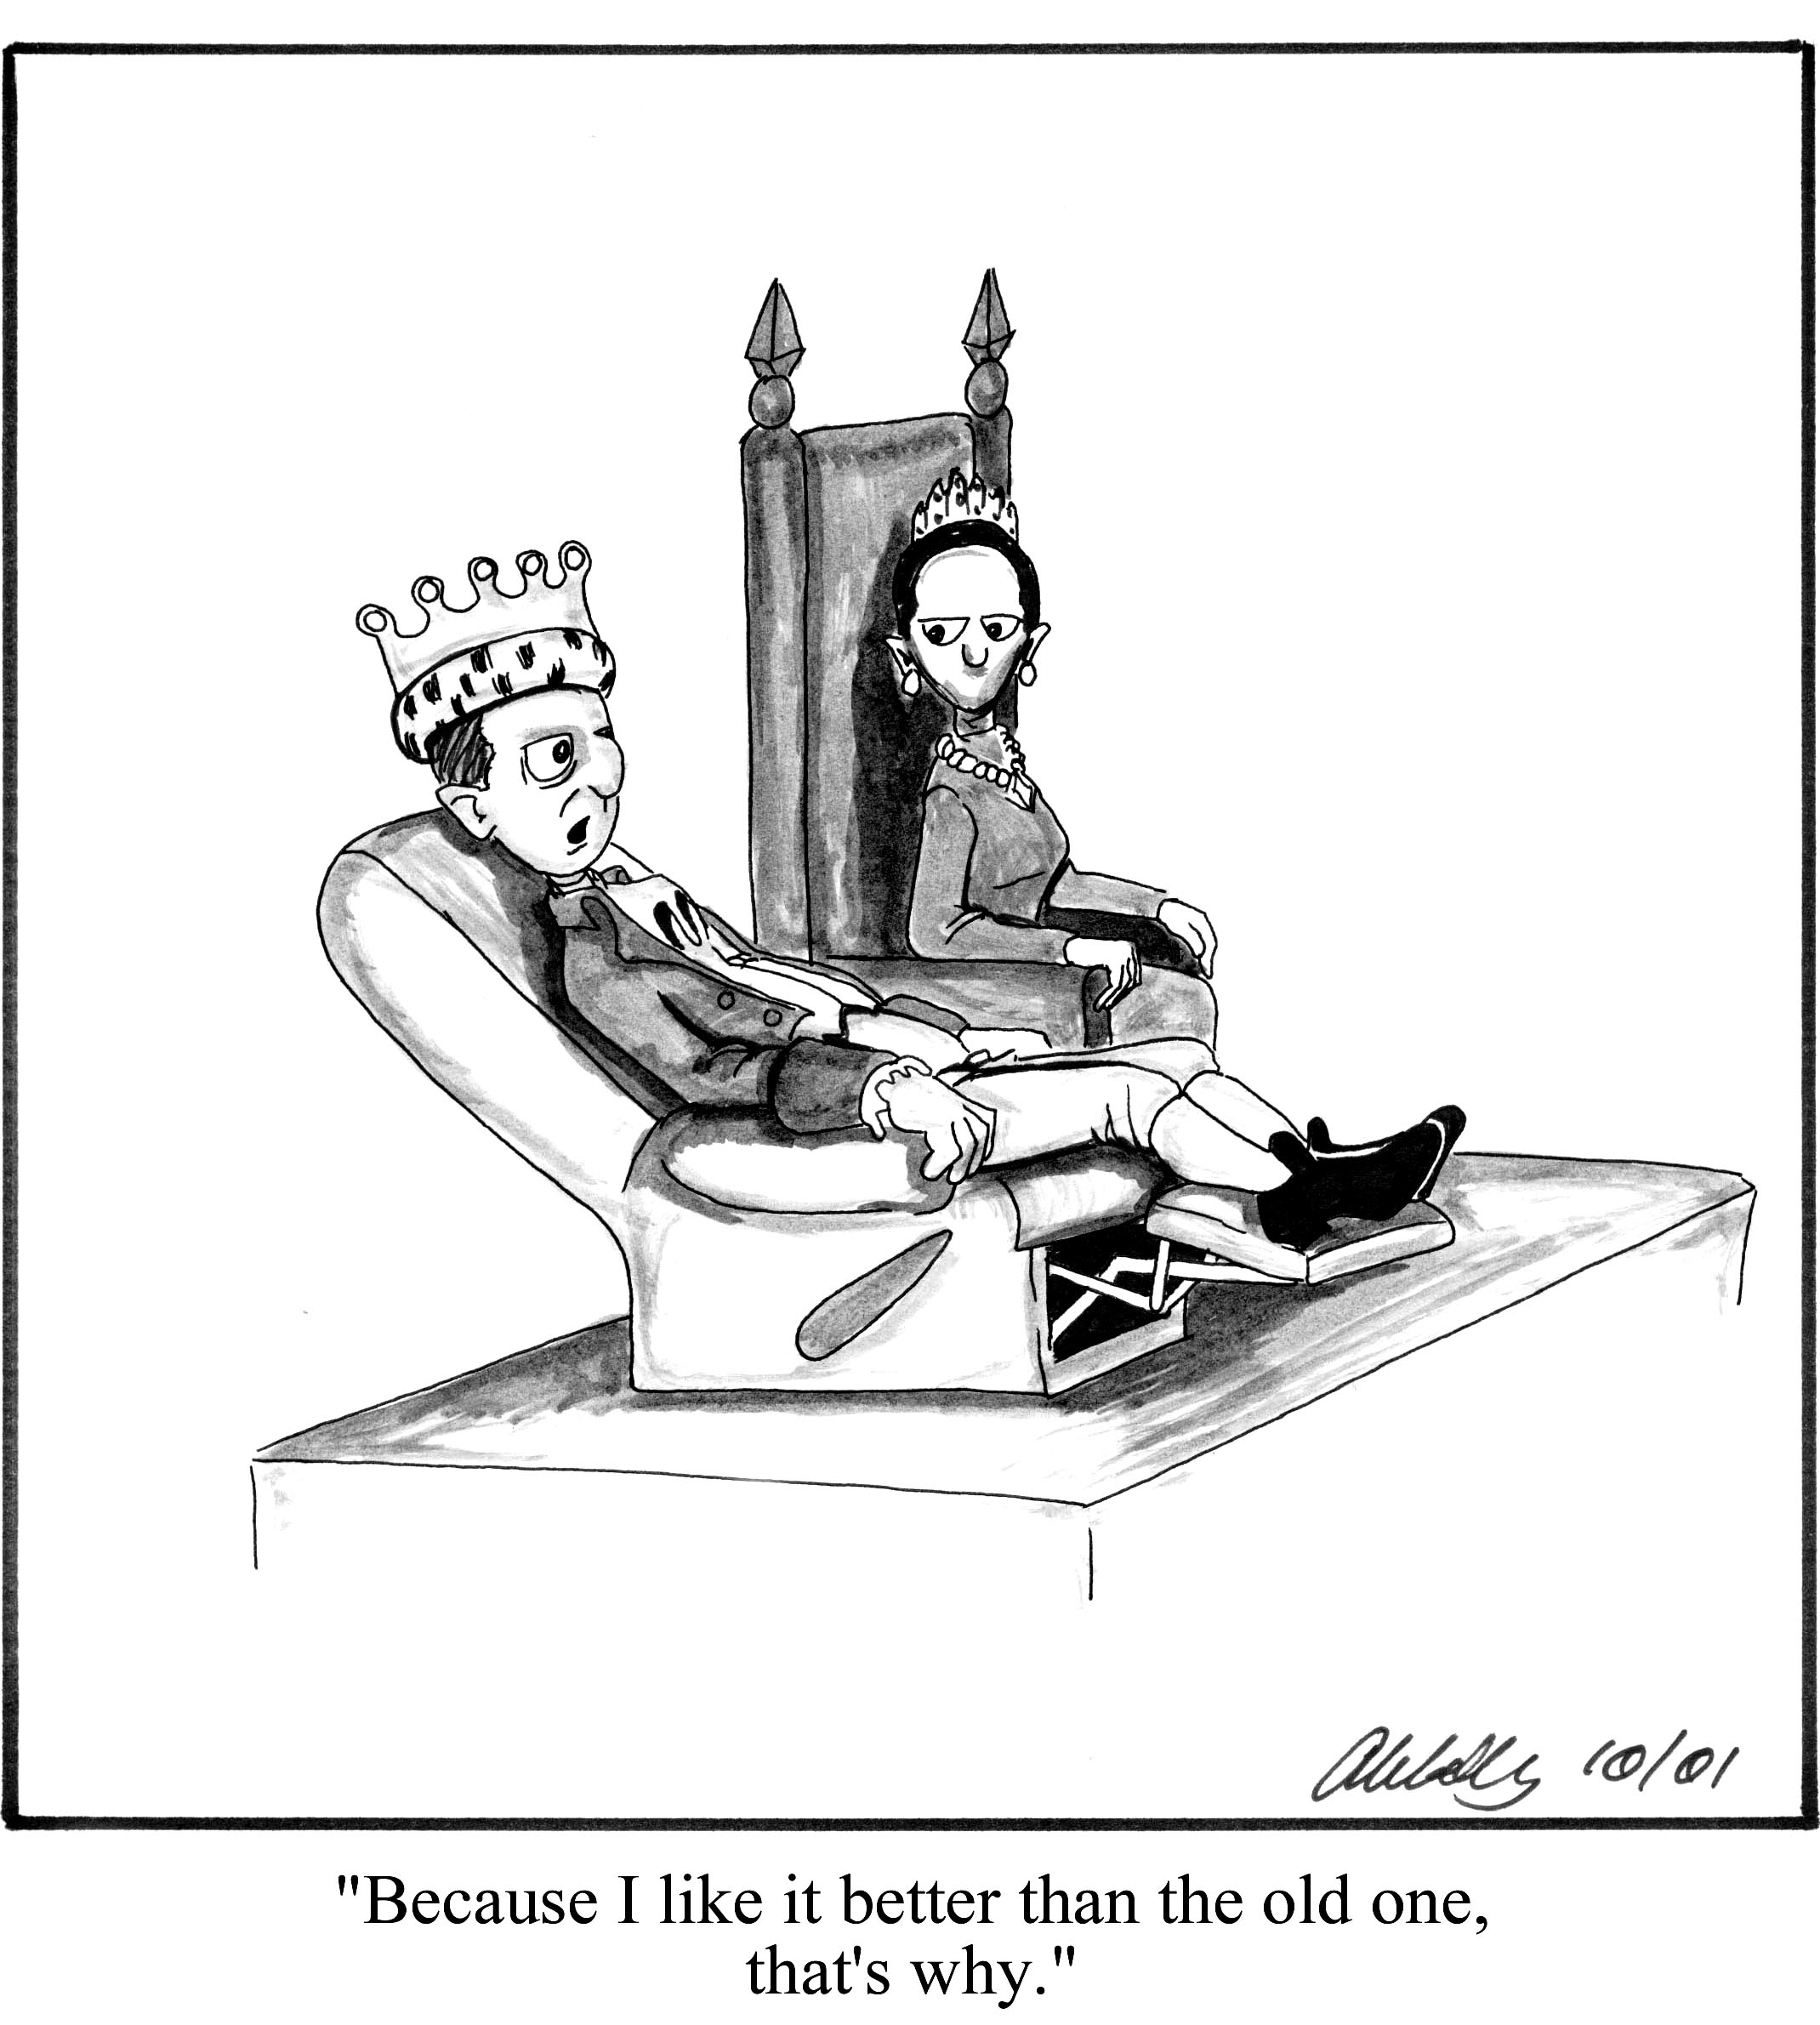
\includegraphics[width=0.5\textwidth]{throneEC.jpg}
  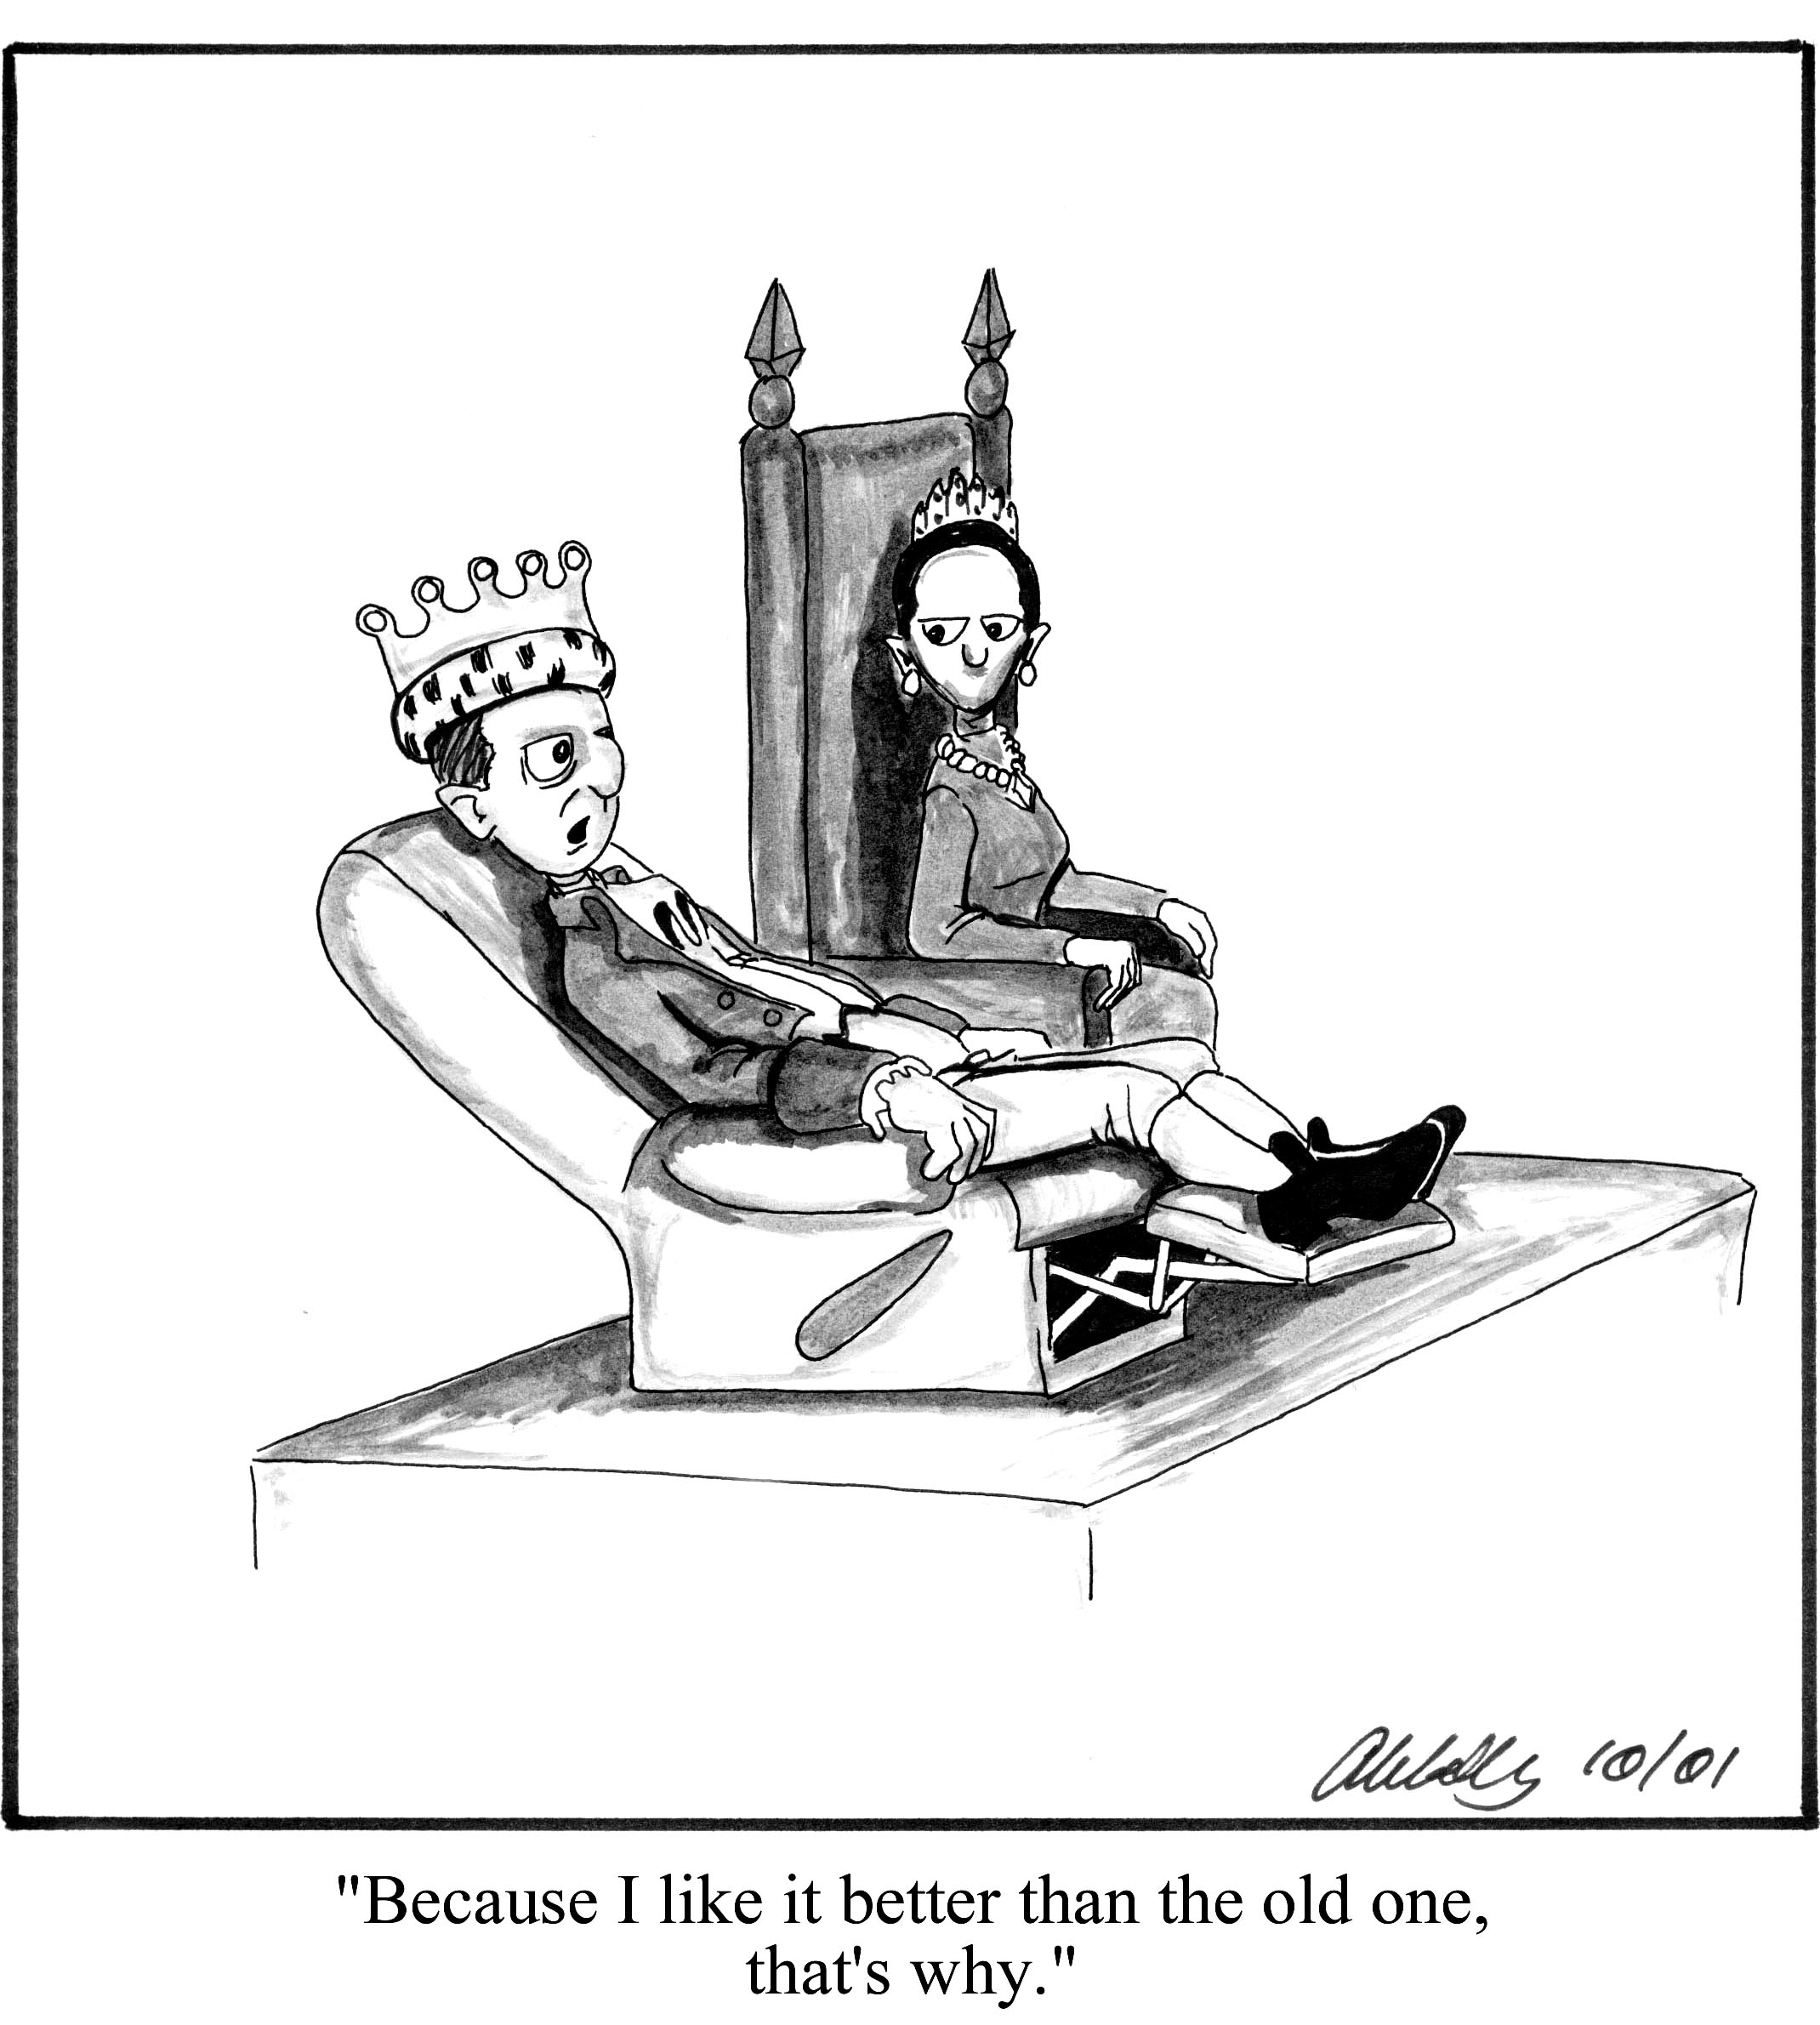
\includegraphics[width=0.3\textwidth]{throneEC.jpg}
  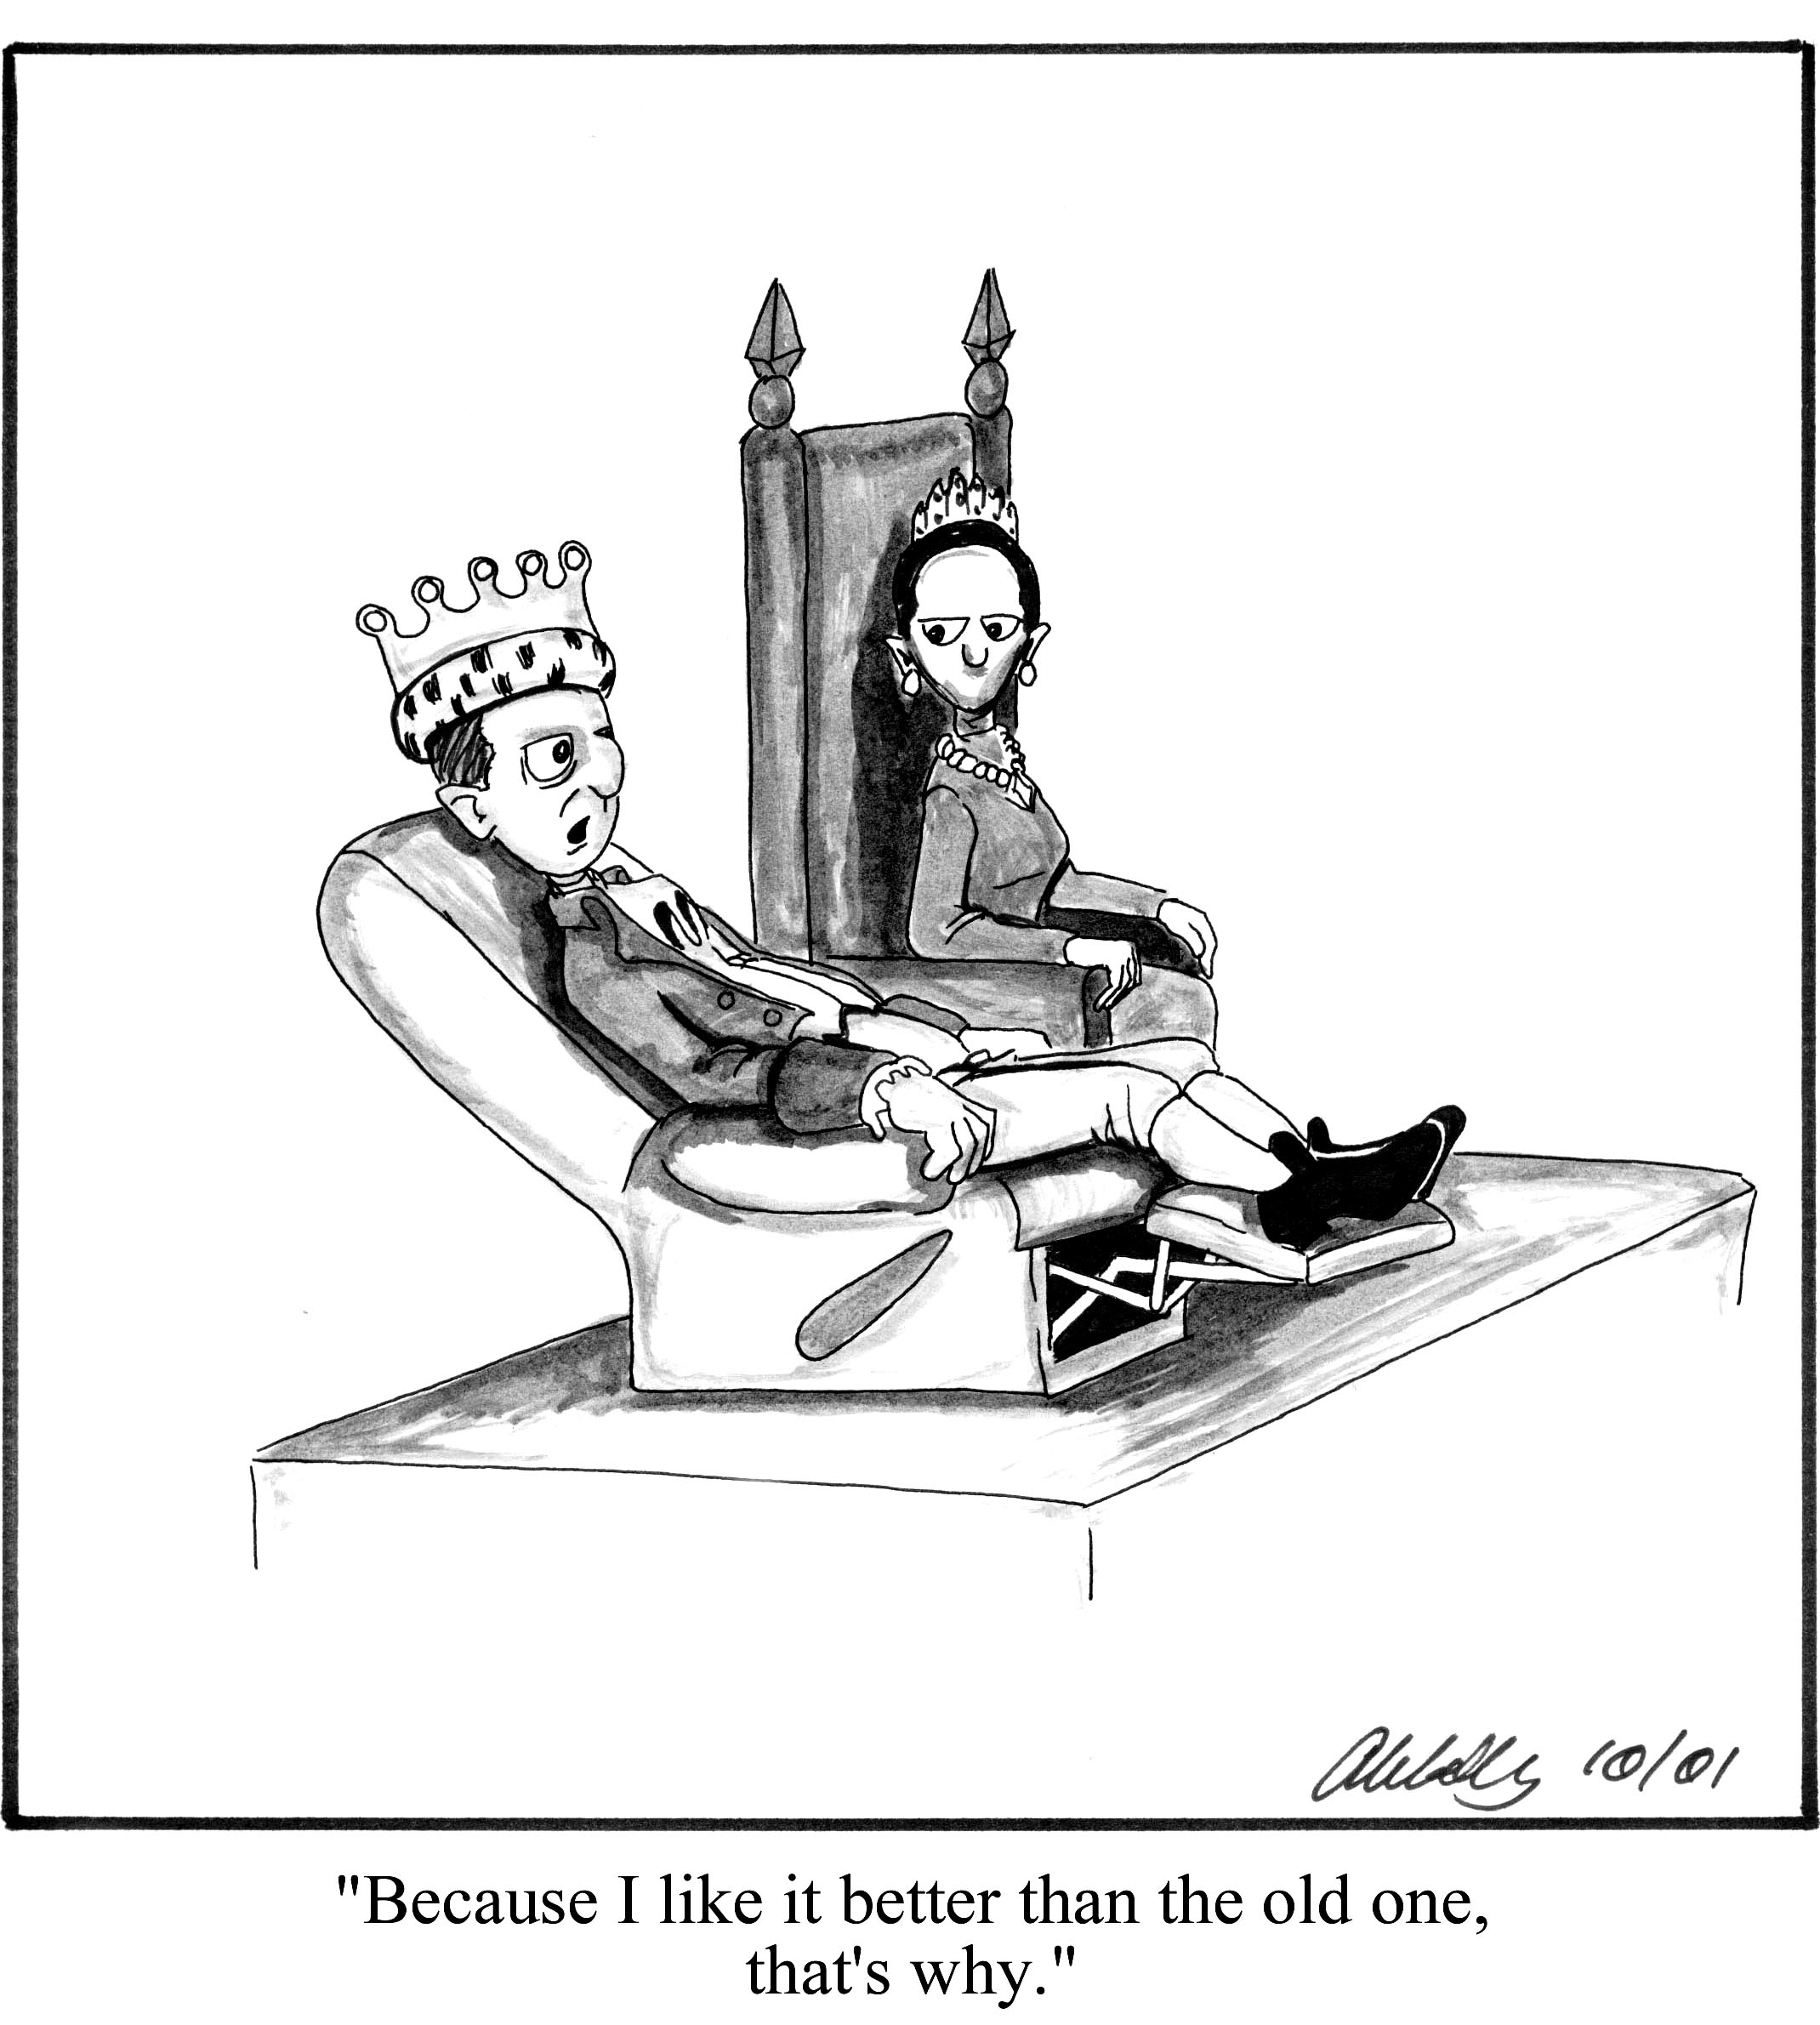
\includegraphics[width=0.15\textwidth]{throneEC.jpg}
\end{verbatim}

%------------------------------------------------------------------------------
% Refs:
%
\label{sect:bib}
\bibliographystyle{plain}
%\bibliographystyle{alpha}
%\bibliographystyle{unsrt}
%\bibliographystyle{abbrv}
\bibliography{easychair}

%------------------------------------------------------------------------------
\appendix
\section{{\easychair} Requirements Specification}
\label{sect:easychair-requirements}

The following high-level requirements were set for the development of
the {\easychair} class, and were refined as development went along.



